\begin{figure}[H]
  \centering
  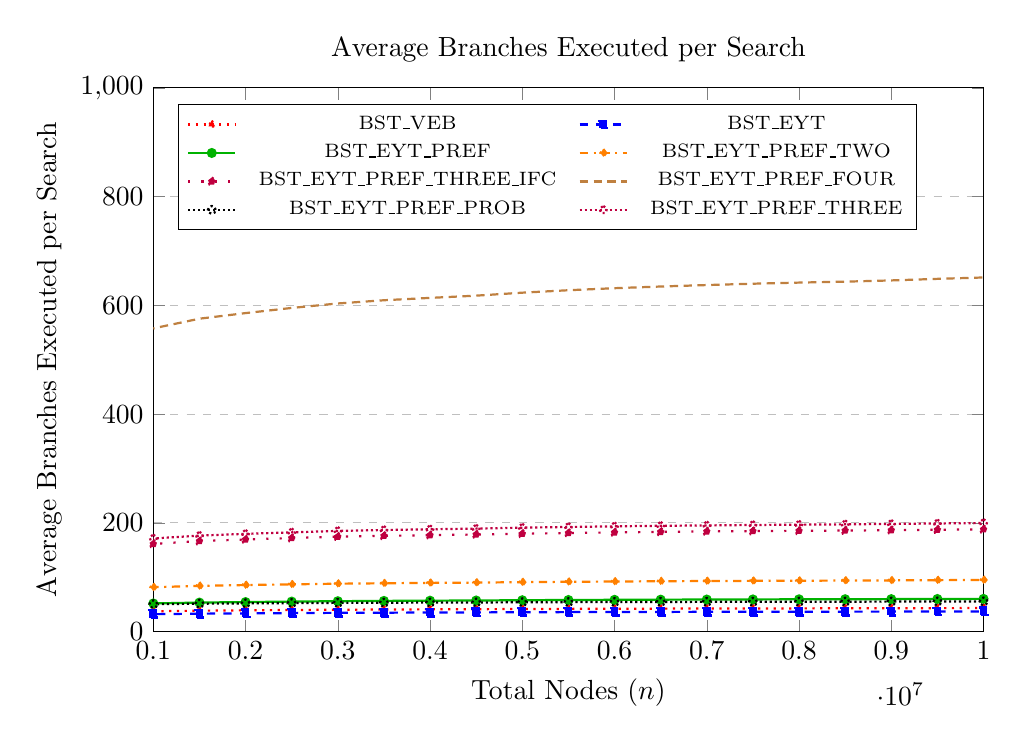
\begin{tikzpicture}
    \begin{axis}[
        title={Average Branches Executed per Search},
        xlabel={Total Nodes ($n$)},
        ylabel={Average Branches Executed per Search},
        width=\textwidth,
        height=0.7\textwidth,
        xmin=1000000, xmax=10000000,
        ymin=0, ymax=1000,
        ymajorgrids,
        grid style=dashed,
        legend columns=2,
        legend pos=north west,
        legend style={font=\scriptsize, column sep=6pt},
    ]

\addplot+[red, thick, dotted, mark=triangle*, mark options={scale=.7,fill=red}]
  coordinates {
    (500000,35.7548)
    (1000000,37.4596)
    (1500000,38.5689)
    (2000000,39.2593)
    (2500000,39.8635)
    (3000000,40.3432)
    (3500000,40.7333)
    (4000000,41.061)
    (4500000,41.3402)
    (5000000,41.6532)
    (5500000,41.9267)
    (6000000,42.1222)
    (6500000,42.3709)
    (7000000,42.5156)
    (7500000,42.6558)
    (8000000,42.8116)
    (8500000,42.9712)
    (9000000,43.076)
    (9500000,43.277)
    (10000000,43.3998)
  };
\addlegendentry{BST\_VEB}

\addplot+[blue, thick, dashed, mark=square*, mark options={scale=.7,fill=blue}]
  coordinates {
    (500000,30.6173)
    (1000000,32.1408)
    (1500000,33.0816)
    (2000000,33.6359)
    (2500000,34.1684)
    (3000000,34.6539)
    (3500000,34.9313)
    (4000000,35.1642)
    (4500000,35.4172)
    (5000000,35.7008)
    (5500000,35.9517)
    (6000000,36.1493)
    (6500000,36.3166)
    (7000000,36.4804)
    (7500000,36.6077)
    (8000000,36.714)
    (8500000,36.8003)
    (9000000,36.9136)
    (9500000,37.0841)
    (10000000,37.2201)
  };
\addlegendentry{BST\_EYT}

\addplot+[green!70!black, thick, solid, mark=*, mark options={scale=.7,fill=green!70!black}]
  coordinates {
    (500000,49.424)
    (1000000,51.9043)
    (1500000,53.4926)
    (2000000,54.4311)
    (2500000,55.3321)
    (3000000,56.0244)
    (3500000,56.5851)
    (4000000,56.9661)
    (4500000,57.3289)
    (5000000,57.8218)
    (5500000,58.2554)
    (6000000,58.5701)
    (6500000,58.845)
    (7000000,59.0827)
    (7500000,59.3068)
    (8000000,59.4954)
    (8500000,59.6695)
    (9000000,59.8461)
    (9500000,60.1188)
    (10000000,60.3164)
  };
\addlegendentry{BST\_EYT\_PREF}

\addplot+[orange, thick, dashdotted, mark=diamond*, mark options={scale=.7,fill=orange}]
  coordinates {
    (500000,77.6266)
    (1000000,81.7322)
    (1500000,84.1925)
    (2000000,85.743)
    (2500000,87.0173)
    (3000000,88.2005)
    (3500000,89.0158)
    (4000000,89.6991)
    (4500000,90.2446)
    (5000000,91.0629)
    (5500000,91.733)
    (6000000,92.2253)
    (6500000,92.7404)
    (7000000,93.0984)
    (7500000,93.4445)
    (8000000,93.6858)
    (8500000,93.9759)
    (9000000,94.3041)
    (9500000,94.7135)
    (10000000,95.0857)
  };
\addlegendentry{BST\_EYT\_PREF\_TWO}

\addplot+[purple, thick, loosely dotted, mark=pentagon*, mark options={scale=.7,fill=purple}]
  coordinates {
    (500000,153.325)
    (1000000,161.387)
    (1500000,166.517)
    (2000000,169.526)
    (2500000,172.167)
    (3000000,174.653)
    (3500000,176.172)
    (4000000,177.422)
    (4500000,178.699)
    (5000000,180.014)
    (5500000,181.433)
    (6000000,182.495)
    (6500000,183.489)
    (7000000,184.302)
    (7500000,184.946)
    (8000000,185.477)
    (8500000,185.98)
    (9000000,186.563)
    (9500000,187.415)
    (10000000,188.144)
  };
\addlegendentry{BST\_EYT\_PREF\_THREE\_IFC}

\addplot+[brown, thick, densely dashed, mark=x*, mark options={scale=.7,fill=brown}]
  coordinates {
    (500000,529.714)
    (1000000,557.707)
    (1500000,575.53)
    (2000000,585.842)
    (2500000,595.301)
    (3000000,603.515)
    (3500000,609.458)
    (4000000,613.797)
    (4500000,617.908)
    (5000000,623.381)
    (5500000,627.871)
    (6000000,631.629)
    (6500000,634.703)
    (7000000,637.393)
    (7500000,639.869)
    (8000000,641.91)
    (8500000,643.644)
    (9000000,645.915)
    (9500000,648.787)
    (10000000,651.351)
  };
\addlegendentry{BST\_EYT\_PREF\_FOUR}

\addplot+[black, thick, densely dotted, mark=o, mark options={scale=.7,fill=black}]
  coordinates {
    (500000,48.9526)
    (1000000,50.4912)
    (1500000,51.4254)
    (2000000,52.0073)
    (2500000,52.5033)
    (3000000,52.9719)
    (3500000,53.27)
    (4000000,53.5151)
    (4500000,53.73)
    (5000000,54.0084)
    (5500000,54.2906)
    (6000000,54.4819)
    (6500000,54.6435)
    (7000000,54.8052)
    (7500000,54.9357)
    (8000000,55.046)
    (8500000,55.1636)
    (9000000,55.2689)
    (9500000,55.4345)
    (10000000,55.5513)
  };
\addlegendentry{BST\_EYT\_PREF\_PROB}

\addplot+[purple, thick, densely dotted, mark=pentagon, mark options={scale=.7,fill=purple}]
  coordinates {
    (500000,162.649)
    (1000000,171.375)
    (1500000,176.616)
    (2000000,179.89)
    (2500000,182.605)
    (3000000,185.255)
    (3500000,186.945)
    (4000000,188.287)
    (4500000,189.52)
    (5000000,191.278)
    (5500000,192.511)
    (6000000,193.684)
    (6500000,194.708)
    (7000000,195.328)
    (7500000,196.181)
    (8000000,196.767)
    (8500000,197.386)
    (9000000,198.126)
    (9500000,198.99)
    (10000000,199.72)
  };
\addlegendentry{BST\_EYT\_PREF\_THREE}

    \end{axis}
  \end{tikzpicture}
  \caption[Average Branches Executed per Search]{The figure includes the average branches which have to be executed for the given implementation per search operation.}
  \label{fig:totalbraches}
\end{figure}
